% intro.tex - Introduction
\documentclass[openright,final,12pt]{memoir}

% set paper size
\setstocksize{20.98cm}{14.8cm}
\settrimmedsize{20.98cm}{14.8cm}{*}
\settrims{0in}{0in}
\settypeblocksize{17.16cm}{10.73cm}{*}
\setlrmargins{2.16cm}{*}{*}
\setulmargins{1.91cm}{*}{*}
\checkandfixthelayout

% import packages
\usepackage{fullpage}
\usepackage{color,fancyvrb,relsize}

% import a new font and use the sans-serif version by default
\usepackage{helvet}
\renewcommand{\familydefault}{\sfdefault}

% latex preferences
\hyphenpenalty=1000
\tolerance=1000

% put chapters and sections in the toc, only number the chapter
\setcounter{tocdepth}{3}
\setcounter{secnumdepth}{0}

\renewcommand{\chaptername}{}
\renewcommand{\thechapter}{}
%in2.16 ou1.91
%wi14.8 hi20.98
% make the pdf have clickable links
\usepackage[
  bookmarks,
  bookmarksopen,
  bookmarksnumbered=false,
  colorlinks,
  pdfpagemode=None,
  urlcolor=black,
  citecolor=black,
  linkcolor=black,
  pagecolor=black,
  plainpages=false,
  pdfpagelabels,
  pdftitle={Git In the Trenches},
  pdfauthor={Peter Savage}]{hyperref}


% title/author/date
\title{Git In the Trenches}
\author{Peter Savage}

% commands.tex - various things we want to use throughout the document, conveniently defined here

% give us a begin{trenches}
\newenvironment{trenches}{\begin{quote}\begin{rmfamily}In the trenches...\\\\}{\end{rmfamily}\end{quote}}


\date{Feburary 2011}

\begin{document}

% preamble stuff
\maketitle
\cleardoublepage
\tableofcontents

% include all the individual chapters
% intro.tex - Introduction
\cleardoublepage
\chapter{Introduction}
\section{How this book works}
Welcome to Git In The Trenches or GITT, a book designed to help you both apply and understand the subtleties of Git, perhaps the most powerful version control system in use today.
This book is not supposed to be purely a technical reference.
If you are looking for something more reference in nature, you should look at ProGit, by Scott Chacon, published by Apress, as it is a wonderfully detailed look at many of the Git commands.
GITT is more of a scenario based book and by reading it, it is hoped that the experiences and scenarios that you encounter will help give ways to apply Git in practical situations.
Git is a hugely powerful system and once harnessed you are most likely going to wonder how you managed without it.

GITT follows the lives of some developers at a fictional company called Tamagoyaki Inc.
They are a small software outfit who write bespoke software for people.
It may be that you work for a company that is very similar to Tamagoyaki Inc and you are looking to implement a version control system for your own company, or it could be that you have been using a version control for a long time and are looking for a helping hand in applying the Git system to your needs.
Regardless of which box you fit into, GITT should provide you with some useful knowledge in a way that is designed to help you remember the scenarios and their associated solutions.

The book will follow the lead developer John, as he works to bring the company into line by implementing a version control system.
It's not something he's ever really used in earnest and he feels a little out of his depth.
It is hoped that your confidence and knowledge about both version control systems, and Git in particular, will grow whilst reading GITT.

The chapters are presented as weeks during the implementation of Tamagoyaki Inc's version control system project.
Each chapter spells a new week in the project and you will follow the life of John and his colleagues as they solve problems and learn tricks of the Git trade.
As well as presenting and solving common issues, the book will also be littered with breakout boxes, intended to tell you exactly what is happening inside Git at each stage.
This is intended to further your knowledge and understanding of this powerful piece of software.
At the end of each chapter are "John's Notes" which should build into a quick reference guide.

After each week, there is also the opportunity for you to delve further into the guts of what has been presented during the week with the \emph{After Hours} sections.
These sections will take the knowledge that you have learned during the week and take it to a much deeper level, often showing diagrammatic ways of how commits take place, or even looking at the contents of files within the repository file structure itself.
These chapters are not meant to scare you, but are presented in the hope that you can reinforce what you have learned through the week by reading through more complex material.

With a system as complex as Git, knowing the commands is often not the only piece of the puzzle.
A good understanding of the underlying system, and how it reacts when you press that all important \textbf{Enter} button is essential if you want to be able to hold your cool in a crisis.
It is rather difficult to break Git.
There are many safeguards in place, but please be aware that you should try all of the items in the book in a test environment first, to ensure they perform, what you expect.

In the text of the book you will find numerous output listings like the one below.
These not only show you the commands that are being run to interact with the Git system, but also the output that you should expect to see.
You output will always differ to that which is in the book, if sometimes only slightly, but the output has been provided so that you can follow what is happening at each stage.

\begin{code}
john@satsuki:~/coderepo$ ls -la
total 36
drwxr-xr-x  3 john john 4096 2011-07-07 19:12 .
drwxr-xr-x 13 john john 4096 2011-07-09 20:02 ..
-rw-r--r--  1 john john   35 2011-07-07 19:12 another_file
-rw-r--r--  1 john john   25 2011-07-07 19:12 cont_dev
drwxrwxr-x  8 john john 4096 2011-07-07 19:17 .git
-rw-r--r--  1 john john    8 2011-03-31 22:15 temp_file
john@satsuki:~/coderepo$
\end{code}

References in the text to commit IDs and branch names will usually be written in \textbf{bold} and words of general interest will be \emph{emphasised}.
Where commands of directory names are referred to in the text, they will be written in a \texttt{monospace} font for easy distinction.
Throughout the book, you may also encounter \emph{callout} boxes, like the one below.

\begin{callout}{Information}{Callout boxes}
These boxes are used to convey extra information, or to more accurately define terminology.
They are there to give you that little bit of extra information.
\end{callout}

With the introduction over, let's first go through a quick setup guide and then find out why Tamagoyaki Inc even needs a version control system in the first place.

% chap1.tex - Week 1
\chapter{Week 1}
\section{Day 1 - ``Things need to change''}
\subsection{Meeting the Team}

If you're already a seasoned version control user, you may want to skip this chapter.  It's kind of like an introduction to why we even need version control systems in the first place.  This chapter looks at Tamagoyaki Inc's requirements and why they choose the VCS that seemed right for them.  Tamagoyaki Inc. create software for turning a standard PC into a media center.  Their product ships to the end user and they rely very heavily on having a good presense at trade shows, in order to bring in sales.  The following conversation describes the events that led up to the defining "We need a VCS!" discussion.

\begin{trenches}
John sat at his desk and looked out of the window.  The rain was drizzling down the pane, but he didn't care.  It was a quiet Monday morning, the release had gone well on Friday and John was just thinking about implementing the new abstraction layer to the database he'd been asked for.  Through the music playing in his headphones he hardly noticed his boss, the chief designer and the CEO approaching his desk.  

``John,'' shouted his boss, Markus, ``get your team into the board room.  Now!''

Things didn't look good. 
 
\begin{center} * * * \end{center}

``So, what we'd like to know John, is just how a bug that was supposed to have been\ldots'' the CEO back-tracked, ``that was demonstrated as being fixed two weeks ago, made it into the final release of the software?''

``I'm sorry,'' John started, before being cut off.

``Sorry doesn't cut it John,'' said the CEO, Wayne Tobi, ``This was almost a major embarrassment for Tamagoyaki Inc.  We need to ensure this doesn't happen again.  The demonstration at the trade show was close to a complete failure.  Luckily someone had the good sense to bring a backup machine.''  He turned to Markus.  ``I want a report on my desk by the end of the day that states what the problem was, how it slipped through our fingers and what safe guards we are going to put into place so that things like this never happen again.''

``Of course sir,'' Markus replied.  He was bright red with his own variety of embarrassment.

The room fell silent and a few minutes of silence passed before the meeting was drawn to a close and John and his team were allowed to leave.

\begin{center} * * * \end{center}

``So, you're telling me that when Simon came back from holiday, he picked up an older copy of the library from the network share and pushed his latest code into that?''  Markus was holding back the anger.

``It appears that way.''  Said John sullenly.

``Oh for crying out loud.  How did this happen?  Why wasn't he using the latest version?  And why didn't QA pick up on it?''  Markus looked across the meeting room at John.  ``John, you need to make sure this doesn't happen again.  Find a solution!''
\end{trenches}

\subsection{The trouble with storage}

It's not like this situation is completely uncommon.  At one point or another most people have managed to pull old code from somewhere and mistakenly use it in place of the latest, up to date, version.  When storing code on network shares or on local disks, it's easy to lose sight of which version is which, no matter how good your naming convention is.  It's like trying to build one of the baked bean puzzles when you have three boxes of them and you tipped all the pieces into one box for simplicities sake.  Not so simple any more is it?

People have a tendency to use folder names which mean something to them.  However it doesn't necessarily follow that this name means something to another developer.  ``Version 2.3 - fixed bug a'' only means something to you if you know what bug a is and something like ``Version 2.3 - fixed bug a(2)'' is even worse.  Unfortunately allowing people to free form type their own descriptive file names will always lead to problems like this.  When these files are stored on a network share, the problem is exacerbated ten fold because there is often no fixed reference point.

So what's the solution?  Well, in a large number of cases version control can make sure that not only is there a defined place for data to sit, and with a defined structure, but also that you have a full history of the code.  Accountability is very important in code development, especially when releasing software to customers.  In some situations a customer will even mandate that the code being developed for them is stored in a version controlled environment.  In this way, the customer can ask when a certain piece of code was edited, or when an addition first entered the code base.

\section{Day 3 - ``A possible solution''}
\subsection{Version Control Nuances}

There are many offerings for version control out there, Git, Mercurial, Subversion, CVS, and Bazaar to name but a few of the open source ones.  Perhaps a more pertinent question is just which version control system to use.  Each of them has their relative advantages and disadvantages, but some will be suited to certain tasks more than others.  Also, it's worth noting that if you are interacting with other pieces of software, or share some development with another set of developers, it is a good idea to enquire to see what they are using.  Usually you'll find collaboration, forking and patching a lot easier if you're using the same version control system as your upstream or partners.

\begin{trenches}
``So really it seems like the only real solution to this problem bar Klaus' suggestions of reducing the workforce to only one developer, thank you Klaus,'' Klaus nodded in acknowledgement back to John, ``is to implement a version control system.''

Markus chewed his lip.  ``I can see where you're coming from here John, but aren't version control systems really expensive?''

``There are a number of open source offerings we could take a look at first,'' piped up a new voice in the discussion, ``some of them are supposed to be pretty good.''

``Let's all go away, take a look at the various pros and cons and reconvene tomorrow to discuss the findings,'' said John.  ``Sound fair?''
\end{trenches}

So now we need to take a look at some various features of version control systems and see what the various advantages and disadvantages are of each.  We are going to focus on Git here primarily, as this is what the rest of the book is all about.  It is assumed that if you are reading this book, you have most likely already made the decision about which version control system you are going to use.  So let's talk about the various features that are prevalent in most version control systems.

\subsection{Distributed Version Control}

Version control systems usually fit into one of two categories; centralised, or distributed.  Git is a distributed version control system.  It has been designed to run almost everything at a local level.  This will become much more clear when we talk about other features of Git a little later on, but for now just understand that Git isn't tied to a centralised repository.  This is super powerful.  No Really!

\subsection{Branching}

Most version control systems offer branching as part of their default features set.  Branching allows developers to create in essence a clone of their repository and mess around with it, safe in the knowledge that they can switch back to the original whenever they need to.  This allows developers the freedom to experiment with all manner of things without being afraid of affecting the original/clean code base.

Git implements branching in a special way.  Most other version control systems implement branching in a way that almost creates a separate repository.  This is slow and cumbersome.  Git's branching method gives developers the ability to create multiple local branches to play with.  Due to it's distributed nature, when pushing code to a more central location for others to pull from, developers can choose which branches they want to push, allowing code to be experimented with privately.

The implementation of branching in Git is fast.  Due to the fact that repositories are stored locally, the speed of creating a local branch is limited only by the speed of the disks on a local machine.

\subsection{Staging}

Git deals with commits differently to most other version control systems by introducing the staging area.  The staging area allows developers to prepare their commits before they are written to the repository.  Why is this useful or any different to any other version control system.  In Git you can make a change to a file, add it to the staging area, and then continue to make changes to that file, even though you have not yet actually committed anything.
It should be noted that it's not absolutely necessary to use the staging area, but it is there for developers wishing to utilise it.

\subsection{Workflow}

Due to the way that Git has been designed, it's possible to use it in practically any work flow you can think of.  Three of the most common workflows are explained below, and Git can work in any of these, making it one of the more versatile systems out there.

\subsubsection{Centralised Workflow}

In a centralised workflow, a single shared repository is used.  Multiple developers pull changes from here into local working copies, work on the local version, and then push it back up to the central location.  

Git handles this workflow just like most other version control systems.  A developer can not push his changes until he has pulled everything up to the latest from the central repository and resolved any conflicts that may arise.

Using the centralised model for the workflow, each developer has the same level of access to the repository and is considered as \textbf{important} as each other.  For smaller teams, this method will work well, but as teams get larger, a centralised method may get tedious.

\begin{figure}[bt]
	\centering
	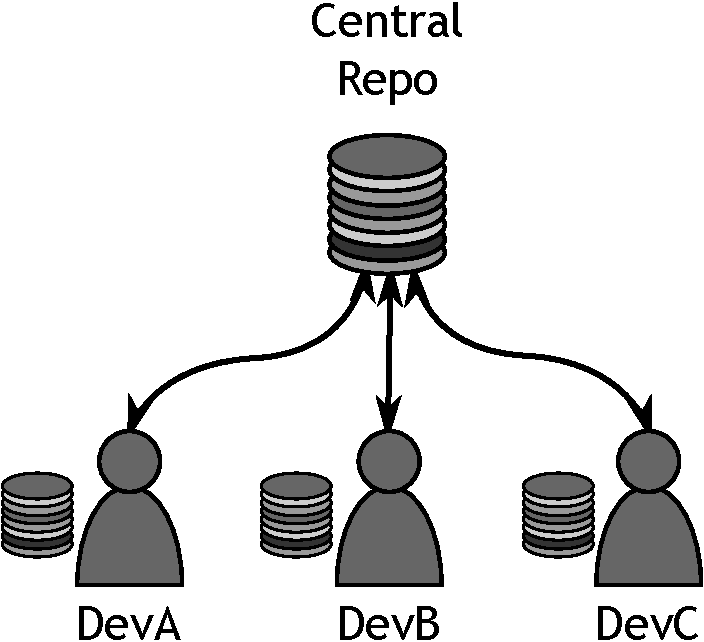
\includegraphics[width=7cm]{images/f-w1-d1.pdf}
	\caption{Centralised Workflow}
\end{figure}

\subsubsection{Integration Manager Workflow}
The integration manager workflow is similar to the centralised workflow because there is still a \textbf{blessed} repository which everyone uses as a reference.  The difference here is that there is only one person who has the rights to push changes to the \textbf{blessed} repository.  This person is referred to as the Integration Manager.  

This workflow is handled exceedingly well by Git.  Developers will work on their repositories locally and then once they are happy, will push their changes to a location where the Integration Manager can see them.  The Integration Manager will then review the changes that the developers have made and will merge them into their own local repository.  Once they are happy that everything is working well, the Integration Manager will push their changes to the blessed repository so that all the other developers can access the changes.

\begin{figure}[bt]
	\centering
	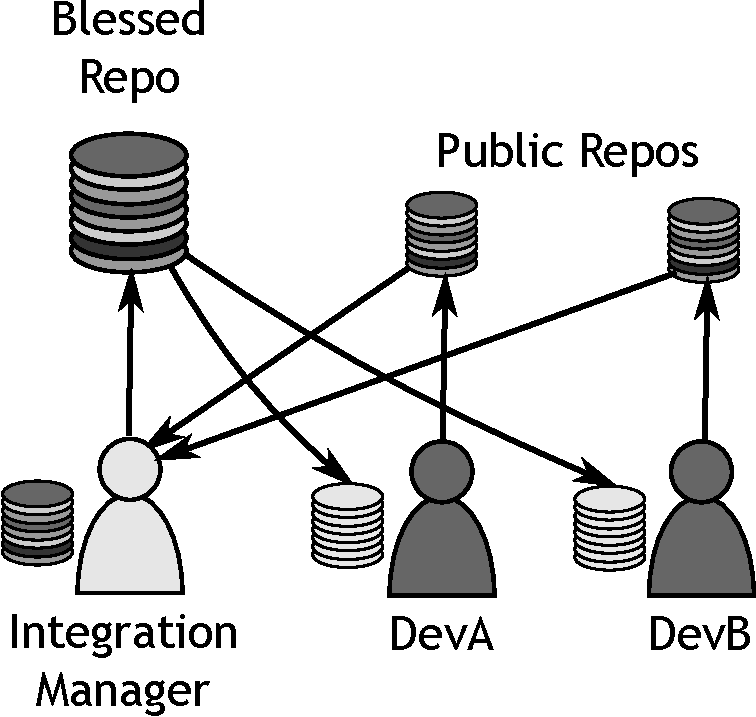
\includegraphics[width=7cm]{images/f-w1-d2.pdf}
	\caption{Integration Manager Workflow}
\end{figure}

\subsubsection{Dictator and Lieutenant Workflow}

The dictator and lieutenant workflow is practically an extension to the integration manager workflow.  It is more suited to larger teams, where modules or sections of the code can be assigned to a \textbf{Lieutenant} who is responsible for blessing all of the changes to that particular section.

Once the Lieutenants are happy with their code, they make it available to the Dictator.  The Dictator then takes on a role similar to the Integration Manager from the previous model.  In the end, all of the changes are pushed to the blessed repository for the developers at the bottom of the tree to pull from.

\begin{figure}[bt]
	\centering
	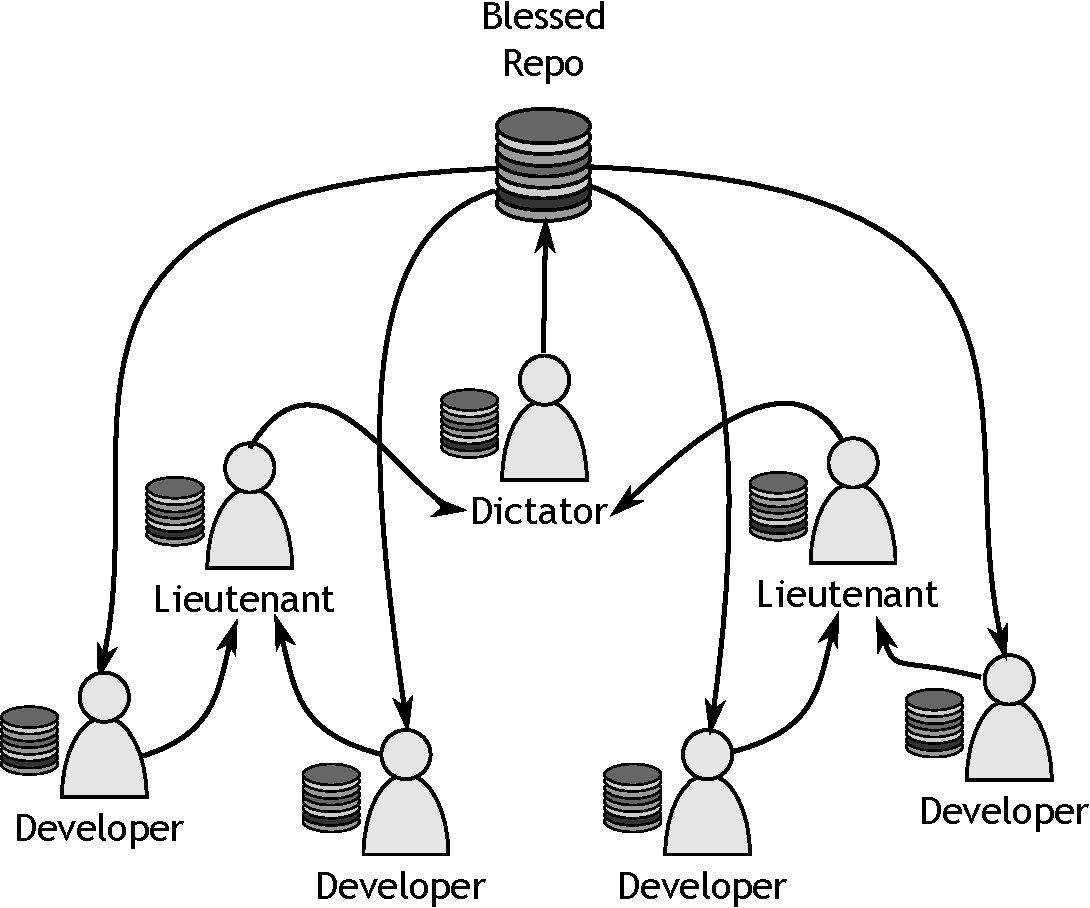
\includegraphics[width=7cm]{images/f-w1-d3.pdf}
	\caption{Dictator and Lieutenant Workflow}
\end{figure}

\begin{figure}[hbt]
\tikzstyle{mybox} = [draw=black, fill=gray!20, very thick, rectangle, rounded corners, inner sep=15pt, inner ysep=20pt]
\tikzstyle{fancytitle} =[fill=black, text=white]
\begin{tikzpicture}
\node [mybox] (box){%
    \begin{minipage}{.9\textwidth}
A blessed repository is one which has the approval of the managers of the project.  The blessed repository is supposed to be the de facto standard where all other clones are made from.  If there is one place where code should be correct, it is the blessed repository.  If you are hosting the project in a public place, the blessed repository will usually be the one that is made available to people as a stable point for developing from.
    \end{minipage}
};
\node[fancytitle, right=16pt] at (box.north west) {Blessed};
\node[fancytitle, rounded corners] at (box.west) {\rotatebox{90}{Terminology}};
\end{tikzpicture}
\end{figure}

The main thing to remember, is that Git can utilise any of these workflows.  This makes it a very flexible system, allowing you to work in whichever way you decide.

\subsection{Offline Committing}

Perhaps one of the most useful and undervalued features of version control systems is that of offline committing.  It may be undervalued because not all version control systems have it.  Offline committing is the ability to continue adding and committing files to the repository without being connected to a centralised repository.  

When travelling or just simply when out of the office, developers and integrators alike are able to continue managing code, viewing histories, viewing diffs and committing changes to their repository.  This is all due to the fact that Git does 99\% of all of it's operations locally.  When a repository is cloned, Git actually sets up a copy of the entire repository locally, giving developers the flexibility to work anywhere, without requiring access to the company network.

When returning to the office, the developers simply push their changes to their ``public'' space, be it local or to a blessed location, and all of the commits that have been made whilst they are away are then made available to the rest of the team, including all history and snapshots.

\subsection{Developer Interaction}

One factor to consider when choosing a version control system, is that of developer interaction.  By this we are referring to the way in which developers use and interact with the version control system itself.  There are four main methods for VCS interaction

\subsubsection{Graphical User Interface Client (GUI)}

A graphical user interface allows the developer, or user, to physically manipulate the repository using a mouse pointer and a graphically rich environment.  A GUI client will typically consist of separate application which is run when a user wants to make changes to a repository such as adding files or committing changes.  

Some developers prefer having a separate client with which to interact with their repository, whilst others prefer to have things integrated a little more.

\subsubsection{Shell Extension Integration}

Shell integration allows the user to interact with their repository using the graphical environment that they would usually use for manipulating files and performing routine directory maintenance.  One of the most common Shell Extensions for Git is the TortoiseGit interface which integrates itself into Windows Explorer, allowing a user to right click on an entity whilst inside a git working tree, and be presented with a context sensitive menu for VCS operations.

\subsubsection{Command Line Interface (CLI)}

The command line interface is favour by many developers as they can script with it and can see exactly what is going on, often in much more detail that with a GUI.  The CLI gives total control over the product and it is worth noting that almost all version control systems start life as command line driven interfaces.  Why is this so?  It can take a lot of time and effort to put all the options and nuances of a system into a GUI.  The CLI will almost always be the most powerful of all tools, especially where version control systems are concerned.

\section{Day 4 - ``A decision is reached''}

\subsection{Analysing Your Requirements}

The most important aspect of choosing a version control system, is to define your requirements.  These can be few, or they can be quite specific, let's see what John and his team decide are the most important aspects for them and ultimately what they decide upon.

\begin{trenches}
``Offline committing seems like it's a pretty useful thing to have.''  Mike said nodding.  ``Especially with people like John travelling all the time.''

``I have to admit, it would be nice to be on the plane, and be able to pull all the code together, knowing all of the history of each section,'' replied John.  ``The branching in Git seems to be quite powerful as well.''

``I must admit,'' chimed in Klaus, ``I've used branching a bit in Subversion before and it was a lifesaver.  It's supposed to be super fast in Git too.''

``And owing to the fact that Git seems to support several workflows, it means we can try them out and see how they work for us.''  Markus looked at the team.  ``Are we settled on Git then?''

The team nodded and everyone walked out of the board room except John.  Things were about to get interesting for him.  Very interesting.
\end{trenches}

Since this book is all about Git, we won't delve too far into the workings or features of other version control systems.  Hopefully, this chapter has given you enough information to go and check out some of the other systems, if you feel the need to.  The main thing to bear in mind is that Git is a Distributed Version Control system.  While this is so, it is equally important to remember that it can be used in the same workflow models as Centralised Version Control systems.

John and his teams requirements are nothing special.  They are a smallish team looking to reap the benefits of having their code in a well organised system.  They are also looking to reorder their team functions and dynamics in order to fit around the version control system and really make it core to their development.  

Version control is not a replacement for workflow.  It is not intended to make everything better.  If you have people going off and doing their own thing and being careless about the way they work, version control is not going to suddenly fix everything.  A tool is just that, a tool and version control is no different.  You can buy the messiest builder in the trade a nice shiny new tool box, but unless they have the mindset to want to change, you'll probably find that all the tools end up in the largest compartment at the bottom.

\section{Day 5 - ``Working like a team''}

\subsection{Team Organisation}

Now that we have the basics dealt with, let's take a little look at how John arranges his team, and see whether version control is going to work for them.  It is important that the team understands how the model should work, what they are expected to do and what level of access they have.  Most of the time people will get more frustrated about not know what they should or shouldn't be doing, rather than that they do or don't have access to certain things.

\begin{trenches}
It was 4:36pm on the Friday and the table in the board room was littered with empty coke cans, pizza boxes and one Japanese bento lunchbox, owned by a particularly stubborn member of the team who had vowed never to eat pizza again.  It had been Marcus' idea to bring in the food reinforcement to help the discussions along.  The team were trying to decide how to organise their model.

``There's nothing to say we can't use a combination of the models is there?'' asked Mike.

``I suppose not,'' said John.  ``What did you have in mind.''  His glasses were slipping down his forehead now and he was getting pretty tired.

``Well, I figure, we basically have the software split into two parts.  We have the library, which myself, Klaus and Jack work on.  Then there's the UI elements which Simon, Martha and Rob handle.  I know there are the tools which Eugene works on too.''  Everyone had started to listen to Mike as he continued.  ``John, you don't want to have to deal with the library component as this more Klaus' space.  So why don't we have two dictators.  Klaus and yourself have access to push up to the blessed repository.  John can pull from his guys, Klaus from his and we end up with an good model for version control.''

John raised his eyebrows, ``Not bad Mike,'' he said, genuinely impressed.  After spending a few hours going through the various models and who was  in charge of what, it felt good to have finally reached a decision.

``So, we start on Monday then?'' asked Markus, who had been listening from the other end of the table.  

``Indeed.''  Announced Klaus, ``Monday we all become Gits!''
\end{trenches}

% chap2.tex - Week 2
\chapter{Week 2}
\section{Day 1 - ``We are coders, we use Git!''}
\subsection{Setting Up the Environment}

So now we are ready to begin delving into and actually using Git, right?  Well, not exactly.
First we have to decide upon how the workflow model we have envisaged is implemented in our version control system.
With Git being so versatile, it's both a blessing and a danger.
It is a good idea to define from early on, exactly how you would like the developers, lieutenants and dictators to behave, before you begin actually committing any code.
Sometimes this isn't possible.
It's quite feasible that you have never used a version control system like Git before and you begin by muddling your way through.
This is normal, but if you are in charge of implementing this type of system for a professional environment, you should really consider first how this is going to work.

Conceptually, the model which was discussed previously is easy to imagine.
We have two dictators, who both have access to the blessed repository and then several developers, who are going to have their changes reviewed and included, by the aforementioned dictators.
The physical representation of the workflow model is summarised in the diagram below.

\begin{figure}[bt]
\centering
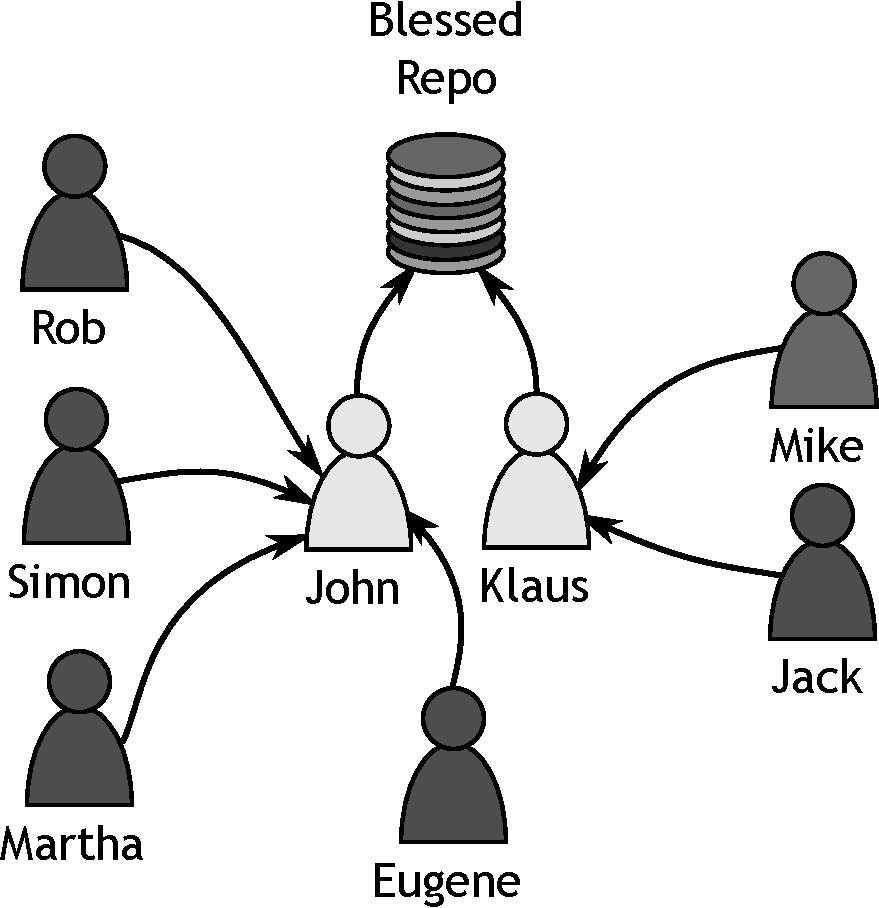
\includegraphics[width=7cm]{images/f-w2-d1.pdf}
\caption{Tamagoyaki Inc's Physical Structure}
\end{figure}

The physical structure is all well and good, but it doesn't determine exactly how the data is moved, just who is responsible for it at each stage in the process.
What is required, is a detailed analysis of where the data flows from and to.
A data flow diagram is useful, but not essential.
However, we will create a slightly different form of diagram to show how the data will be moved from one person to another.
Before we go ahead and look at the diagram, let's go back to the trenches to see how the guys are coping with their repository design.

\begin{trenches}
``John, why are we all sat in here at 9:45am on Monday morning.''  Klaus whined.
``I haven't even ingested enough coffee to check emails yet, let alone meet with people.''

John grinned, ``I don't think any amount of coffee will help you there Klaus, it's your winning personality that will pull you through.''  The rest of the team laughed and then subsided as John started drawing furiously on the board.
``So we have our physical model.
We know which people are going to be in charge of things, but we don't know yet how to arrange our repositories.''

``Good point,'' chimed Mike.

``So.
Obviously we're going to have a blessed repository,'' said John, drawing a circle on the board.
He stepped back, one hand on chin.
``Then I would imagine Klaus and I will have clones of that repository on our local machines.
We will then modify those and push our changes back up to the central copy.''

``I thought Git didn't have a central copy?'' asked Martha.
There were other moans and grunts.

``Well,'' said John, ``as far as I understand it, it doesn't.
I mean Klaus and I will have local copies of the repository too.
We will work on those and then sync our changes back to the server.
It's a sync, moreover a copy.
I think it's actually called a clone.''  He nodded to himself, ``And, since Klaus and I will hardly ever overlap on code, we shouldn't ever need to merge or deal with an conflicts.''

``But what about us monkeys?'' asked Martha, ``Where do we get our clones from?''

``From the central server of course,'' Rob stated smiling.

``Yes,'' John said, ``but I think what Martha is trying to say, is how will you get your updates?''  He started to walk around the room, and one or two of the developers followed him as he reached the windows and leant on the sill.
``I guess you would merge your branch with the blessed one.''

The room went silent and the only noise that could be heard was the rattling of the air conditioner in the ceiling above.

Simon spoke out, ``Well, I was reading over the weekend about this thing called rebase and how in some cases a rebase is better than merging.''

``What's rebase and how is it different to merging?'' asked Mike.

``Well, rebasing is pretty darn clever.
Think of it this way.
You have an upstream branch, in this case, our blessed repository.
You are happily making changes.
When the upstream changes, you could merge the changes in from blessed.
If you do this, you create a single commit which merges the changes in.
It works, but\ldots'' he trailed off a little, ``it can cause problems in certain instances.
A better way to handle it is with rebasing.
Rebasing can take all the changes you have made, squirrel them away, pull down all the changes to bring it up to date, and then whack your changes on top.''

John breathed out, ``It sounds pretty cool Simon, but one thing is abundantly clear, we need to learn more about the Git basics before we start delving into this merging and rebasing.
Let's spend the rest of the day playing with some test repositories and reconvene tomorrow.''
\end{trenches}

If you've never played with a version control system before it is a good idea to take some time to just play.
Pretty soon you'll have learnt the basics and will be in a position where you will want to put your newly honed skills into practise.
Though playing on test repositories is good, it is quite usual that you need to actually use the system in a real environment before real problems arise.
The rest of this chapter is a very quick introduction to Git.
It is presented as an introduction, because it is hoped and expected that the you will take some time out to get to know the system and how it works.

\subsection{Initialising A Repository}
The first thing we need to do is to understand two very important things:

\begin{enumerate}
  \item How to create a Git repository
  \item What a Git repository actually is
\end{enumerate}

The first of these is relatively easy to perform.

\begin{Verbatim}
john@satsuki:~$ mkdir coderepo
john@satsuki:~$ cd coderepo/
john@satsuki:~/coderepo$ git init
Initialized empty Git repository in /home/john/coderepo/.git/
john@satsuki:~/coderepo$
\end{Verbatim}

What we've done here is create a new directory called coderepo, moved into it, and then run the \indexgit{init} command.
The result of this command is a new directory in the coderepo directory called \texttt{.git}.
This directory will hold a local copy of our entire repository.
This will allow us to create branches, merge changes, rebase things and ultimately push our changes to somewhere else.

Something that is crucial to the running of a repository, whether you are an administrator of Git, or a developer who is using it, is an understanding of how Git works.
It is fine to jump in and play with the repository and test the water, but before committing to using Git in a production environment, you should understand what Git actually does in the background in some detail.

During the writing of this book several people have told me that Git is one of the only version control systems where a good understanding of how the underlying system works is not just highly recommended, but bordering on essential.

Let us take a few minutes to talk about how Git works internally and how the data is actually stored.
Git doesn't store changes to files, but actual snapshots of files at specific points in time.
It refers to these by running an \index{SHA-1}SHA-1 hash against the file.
By doing this, it is easy to Git to detect if a file has changed.
If the SHA-1 hash of a file changes, then the file must have been modified.

When a commit is made to the repository, Git stores a few things.
A \index{commit}commit object is created.
This contains information about who made the commit, the parent of the commit and points to a tree object.
The tree object describes what the repository looked like at the time of the commit.
In other words the tree object, tells Git what files were in there.
Lastly, Git stores the files that were in the repository under their SHA-1 names in the objects directory.
Of course Git is super clever here because if you have exactly the same file in multiple commits, the SHA-1 hash of that file doesn't change and therefore Git only stores one copy of the file to save space.

The commit object is also referred to by an SHA-1 hash.
This is different to many other version control systems which use either a number that refers to the repository or a per file version number.
Getting used to seeing 40 character SHA-1 hashes can take a little time.
Saying "I need the commit referred to as  bf81617d6417d9380e06785f8ed23b247bea8f6d," is certainly not as easy as saying you need revision 6.
However, Git handles these hashes well, and you can reference a commit using a few of the characters from the beginning, as long as those characters uniquely refer to that commit, i.e., as long as your choice isn't in any way ambiguous.

\section{Day 2 - ``Making commitments''}
\subsection{Let's Make a Repository}

The most simple way of committing a file into the repository is to create it, or bring it into your working copy and use the commands below.

\begin{Verbatim}
john@satsuki:~/coderepo$ touch my_first_committed_file
john@satsuki:~/coderepo$ git add my_first_committed_file
john@satsuki:~/coderepo$ git commit -m 'My First Ever Commit'
[master (root-commit) cfe23cb] My First Ever Commit
 0 files changed, 0 insertions(+), 0 deletions(-)
 create mode 100644 my_first_committed_file
john@satsuki:~/coderepo$
\end{Verbatim}

What we have done here, is to create a new blank file and add it into the repository using the \indexgit{add} command.
Then we have committed it into the repository using the \indexgit{commit} command.
Let's make a few changes to our working copy and see what the result is.
First we are going to add another two new files, then we are going to make changes to our original file and finally we are going to run git status to see what Git has to say about our changes.

\begin{Verbatim}
john@satsuki:~/coderepo$ echo "Change1" > my_first_committed_file
john@satsuki:~/coderepo$ touch my_second_committed_file
john@satsuki:~/coderepo$ touch my_third_committed_file
john@satsuki:~/coderepo$ git status
# On branch master
# Changed but not updated:
#   (use "git add <file>..." to update what will be committed)
#   (use "git checkout -- <file>..." to discard changes in
 working directory)
#
#	modified:   my_first_committed_file
#
# Untracked files:
#   (use "git add <file>..." to include in what will be
 committed)
#
#	my_second_committed_file
#	my_third_committed_file
no changes added to commit (use "git add" and/or "git
 commit -a")
john@satsuki:~/coderepo$
\end{Verbatim}

So we can see that \indexgit{status} is reporting that there are changes to our first committed file, and that our second and third files are \textbf{untracked}.
\index{untracked!files}Untracked files are ones which Git detects as being present in the working directory, but which haven't yet been added and there for upon running a commit, these files will not be added to the repository.
Notice that if we tried to run a commit now, nothing would actually be committed to the repository.
Even though there are changes to to my\_first\_committed\_file, we have not asked Git to include these.
So, let's go ahead and do that, and at the same time we'll make a few changes to my\_second\_committed\_file, and add those too.

\begin{Verbatim}
john@satsuki:~/coderepo$ git add my_first_committed_file
john@satsuki:~/coderepo$ echo "Change1" > my_second_committed_file
john@satsuki:~/coderepo$ git add my_second_committed_file
john@satsuki:~/coderepo$ git status
# On branch master
# Changes to be committed:
#   (use "git reset HEAD <file>..." to unstage)
#
#	modified:   my_first_committed_file
#	new file:   my_second_committed_file
#
# Untracked files:
#   (use "git add <file>..." to include in what will be
 committed)
#
#	my_third_committed_file
john@satsuki:~/coderepo$
\end{Verbatim}

Now we can see that one of the sections has changed to "Changes to be committed".
So this means that Git has recognised and remembered that we are expecting these files to be committed when we next run a \texttt{git commit}.

\subsection{Committing the Uncommitted}

\begin{trenches}
``John, what is going on here?'' shouted Klaus from across the hallway.
The entire office had heard Klaus banging his hands down on the desk for the last fifteen minutes.
``John!'' the shout turned into a scream.

``Calm down Klaus, I'm just coming.''  John walked over to Klaus and pulled up one of the folding plastic chairs.
After a few minutes of fumbling he finally managed to take up his position next to an infuriated Klaus.

``John, Git is driving me crazy.
I have added files to the repository and I keep running a commit, but the changes aren't getting put into the blasted repo.''  Klaus was clearly distressed and John resisted the urge make jokes.

John pointed at the screen.
``Run a git status Klaus and I'll show you what the problem is.''
\end{trenches}

To understand what Klaus was getting in a spin about, let's make a change to my\_second\_committed\_file now and see how this affects things.
Remember we have already added the file, but we haven't yet made a commit.

\begin{Verbatim}
john@satsuki:~/coderepo$ echo "Change2" >>
 my_second_committed_file
john@satsuki:~/coderepo$ git status
# On branch master
# Changes to be committed:
#   (use "git reset HEAD <file>..." to unstage)
#
#	modified:   my_first_committed_file
#	new file:   my_second_committed_file
#
# Changed but not updated:
#   (use "git add <file>..." to update what will be
 committed)
#   (use "git checkout -- <file>..." to discard changes in
 working directory)
#
#	modified:   my_second_committed_file
#
# Untracked files:
#   (use "git add <file>..." to include in what will be
 committed)
#
#	my_third_committed_file
john@satsuki:~/coderepo$
\end{Verbatim}

How interesting!  We now have three sections and one of our files appears twice under both Changes to be committed and Changed but not updated.
What does this mean?  If you remember back, we spoke about a \index{staging}staging area.
This is one area in which Git differs to many version control systems.
When you \textbf{add} a file into the repository, Git will actually make a copy of that file and move it into the staging area.
If you then go ahead and change that file, you would need to run another git add in order for Git to copy your changed file into the staging area.
The most important thing to remember is that Git will only ever commit what is in the staging area.

So, if we go ahead and run our commit now, we will only have the changes marked in Changes to be committed appearing in our repository.

\begin{Verbatim}
john@satsuki:~/coderepo$ git commit -m 'Made a few changes to
first and second files'
[master 163f061] Made a few changes to first and second files
 2 files changed, 2 insertions(+), 0 deletions(-)
 create mode 100644 my_second_committed_file
john@satsuki:~/coderepo$
\end{Verbatim}

In our examples, we have used the syntax \texttt{git commit -m 'Message'}.
This is a slightly special way of committing, it allows us to specify our commit log message on the command line.
If we wanted to, we could run the command git commit and this would open a text editor that we could use to input our commands.

Let us finish off our round of committing by using the \texttt{git commit -a} option.
This commits all of the changes to files which are already tracked.
Consequently we do not have to specify the files with \texttt{git add}, like we have had to previously.
Any file which has been modified and has previously been added to the repository, will have it's changes committed upon running that command.

\begin{Verbatim}
john@satsuki:~/coderepo$ git status
# On branch master
# Changed but not updated:
#   (use "git add <file>..." to update what will be committed)
#   (use "git checkout -- <file>..." to discard changes in
 working directory)
#
#	modified:   my_second_committed_file
#
# Untracked files:
#   (use "git add <file>..." to include in what will be
 committed)
#
#	my_third_committed_file
no changes added to commit (use "git add" and/or "git commit
 -a")
john@satsuki:~/coderepo$
\end{Verbatim}

\begin{Verbatim}
john@satsuki:~/coderepo$ git commit -a -m 'Finished adding
 initial files'
[master 9938a0c] Finished adding initial files
 1 files changed, 1 insertions(+), 0 deletions(-)
john@satsuki:~/coderepo$
\end{Verbatim}

\begin{Verbatim}
john@satsuki:~/coderepo$ git status
# On branch master
# Untracked files:
#   (use "git add <file>..." to include in what will be
committed)
#
#	my_third_committed_file
nothing added to commit but untracked files present (use
"git add" to track)
john@satsuki:~/coderepo$

\end{Verbatim}

\section{Day 4 - ``Let's do this right, not fast''}

\subsection{Uh-Oh I Think I Made A Mistake}

So now we are fairly well acquainted with adding files into the repository and performing commits.
In a short while we will learn about how to view the changes we have made and perform diffs against various objects.
Before we close out the week, we need to go back to the trenches one last time.

\begin{trenches}
``Rob, ya got a second?'' asked Mike.

``Sure, what's up?'' replied Rob from across the office.
``Gimme two secs to make this commit.''  The office went silent again whilst Rob's fingers darted across the keyboard.
``Ahh.
Damn it!'' shouted Rob.

Mike rose from his chair and walked over to Rob.
``What's up?''

``I just added a file into the staging area, but I don't want it there.''  He shook his head, ``Well not yet anyway.''

Mike chuckled, ``Sorry for interrupting dude.''

``Nah, it's OK, I just need to know how to pull this file out of the index.''

``Git reset,'' shouted a voice.
The stillness of the office was interrupted by a chair free wheeling across the floor.
The occupant of the chair was Klaus.
He seemed proud that he was finally getting to grips with things.
``You can use git reset to reset a file that's in the index.''  He grabbed at the keyboard, ``Here, lemme show you.''
\end{trenches}

The git reset is great at removing things from the index that you don't want to be there.
Of course, it can do a great many other things, but for now, let us concern ourselves with the scenario presented above.
We are working away, and have added a number of files into the index ready for committing, when we discover that we are actually not ready to commit them.
In the following example, we are going to add the file my\_third\_committed\_file and then remove it from the index.

\begin{Verbatim}
john@satsuki:~/coderepo$ git add my_third_committed_file
john@satsuki:~/coderepo$ git status
# On branch master
# Changes to be committed:
#   (use "git reset HEAD <file>..." to unstage)
#
#	new file:   my_third_committed_file
#
john@satsuki:~/coderepo$
\end{Verbatim}

Notice how my\_third\_committed\_file is now ready to be committed to repository.
The problem is we need to add something more to it before we do.
Remember that when we run the git add command, we are copying the file from our working copy to the index.
If we decide we no longer want that file in the repository, we can run the following.

\begin{Verbatim}
john@satsuki:~/coderepo$ git reset my_third_committed_file
john@satsuki:~/coderepo$ git status
# On branch master
# Untracked files:
#   (use "git add <file>..." to include in what will be
 committed)
#
#	my_third_committed_file
nothing added to commit but untracked files present (use
 "git add" to track)
john@satsuki:~/coderepo$
\end{Verbatim}

We have discarded the file which was residing in the index.
This is very important to note.
We are not moving the file from the index back into our working directory, we are literally just deleting the file from the index.
Our working copy remains unaffected.
We could run the \indexgit{reset} command without appending a file.
If we did this, all the files in the index would have been discarded.

\begin{trenches}
``So, I think we are all agreed, I'll keep a version of the repository under Git version control.
Until everyone else feels comfortable with some of the more advanced features.''  John looked around the room for any disagreements but there were none.

``Agreed John,'' said Markus, ``I'm pleased with how you guys are progressing, very pleased, but like John said, it's far better for us to take our time and to implement this correctly, than to rush it and to end up with something that we can't administrate and that we don't know how it works.''

``So next week, I want you all to start playing with diffing and logs and don't forget we have an important release due too.''  John pushed his glasses further up his nose.
``The week after that we'll start looking at branching and by then we may be at the stage where we can implement our model.''

Everyone nodded in agreement.
\end{trenches}

\begin{callout}{Knowledge}{How do we change the commit message editor?}\index{changing!commit editor}
We spoke earlier about the configuration file and how it stores information about our Git instance.
Git can use any text editor you require, even a graphical one, though the need rarely arises.
As mentioned earlier, Git has a preference lever when talking about configuration.
First and foremost it will look in the repositories own 'config' file in the .git folder.
Then, it will look in the users \texttt{\textasciitilde/.gitconfig} file.
Finally, Git will look in your distributions own global folder.

If we wanted to change the editor that Git would use to modify commit messages, we can either modify the files directly, or run a command similar to the following;

\begin{Verbatim}
git config core.editor "nano"
\end{Verbatim}

If we want the changes to apply globally, meaning it would affect all repositories we administrate as this user, unless overridden by a repository setting, we would run the following;

\begin{Verbatim}
git config --global core.editor "nano"
\end{Verbatim}

It is worth noting that you can also use the \$EDITOR environment variable to accomplish the same thing.
Many people use this in preference to the modifying the Git configuration simply because many other programs honour this setting.
\end{callout}

\index{files!moving}\index{files!deleting}\index{files!adding}Now we know how to add files into the repository.
The question is, what do we do if we need to remove a file, or even rename it.
Well, git has some commands to help with that.
\indexgit{rm} and \indexgit{mv} delete and move files respectively.
Usually when you want to remove files from the repository, or move them, this is how you will handle it, but what if you have already deleted a tracked file manually?  Well, you have two options.
You could run \texttt{git commit -a}, but remember this will commit all changes to tracked files.
You could also run a \texttt{git rm <filename>} with the name of the file you have just deleted.
Git will then push that change into the staging area ready for commit.
The same applies to moving a file

However, it is worth noting something in the way that Git handles renames.
Git does not track renames explicitly.
This means that by running the \texttt{git mv <source> <dest>} command, you are essentially running a Linux \texttt{mv} command, followed by the \texttt{git rm} on the source file and \texttt{git add} on the destination file.
Running the \texttt{git mv} command is a shorthand way of doing just that.
It is worth playing with this to ensure that you understand what is happening.
As an exercise, inspect the repository after each command so that you understand at what point Git recognises your actions as a rename.

We have run through a few basic commands in Git.
If you are familiar with version control systems, then possibly the only real difference you will have noticed is that of the staging area.
It really is powerful, and allows you to organise and prepare your commits, so that they are both meaningful and coherent.

For Tamagoyaki Inc, their plan to implement version control was far too aggressive.
Most of the members of the team had never even used a version control system.
When deciding to implement version control, it is essential to ensure that you are doing it for the right reasons.
Version control is a tool to help you to keep things in order, but remember tools are nothing without process.
It is process that is key to the order.


\clearpage
\section{Summary - John's Notes}
\subsection{Commands}
\begin{itemize}
\item\texttt{git add} - Add files into the index or staging area

\item\texttt{git commit } - Commit files into the repository, using text editor for commit message

\item\texttt{git commit -m '<Message>'} - Commit files into the repository, using the command line to supply commit message

\item\texttt{git commit -a} - Commit all tracked files into the repository that have changed, using text editor for commit message

\item\texttt{git reset <path>} - Remove file from index or staging area

\item\texttt{git status} - Show the status of tracked, changed, untracked files
\end{itemize}

\subsection{Terminology}
\begin{itemize}
\index{Terminology!Branch}\item\textbf{Branch} - A way of working on the same set of code in parallel without modifications overlapping

\index{Terminology!Commit}\item\textbf{Commit} - A group of objects and a tree in a Git repository
\end{itemize}

% chap3.tex - Week 3
\cleardoublepage
%\phantomsection
\chapter{Week 3}
\section{Day 1 - ``But how do I see what's going on?''}
\subsection{Logging in Git}

Perhaps the best feature of a version control system is the level of accountability that it offers if set up correctly.  What do we mean by this?  People often mistake the word \textbf{accountability} for the word \textbf{blame}.  This is not true at all.  Accountability is key in understanding the events that led up to a particular bug being introduced, or a situation occurring.  How this is dealt with, is a up to the management teams, but accountability should not be something that is revered, it should be something that is looked upon as a tool to help define the cause of a problem.

By its very nature, a version control system is also a logging system.  Every time we committed something into the repository in the last chapter, we supplied a log message.  In fact, if we don't supply a commit message, let us see what happens.

\begin{Verbatim}[frame=leftline,framerule=1mm,fontsize=\relsize{-3}] 
john@akira:~/coderepo$ git status
# On branch master
# Untracked files:
#   (use "git add <file>..." to include in what will be 
committed)
#
#	my_third_committed_file
nothing added to commit but untracked files present (use "git 
add" to track)
john@akira:~/coderepo$ git add my_third_committed_file
john@akira:~/coderepo$ git commit -a -m ''
Aborting commit due to empty commit message.
john@akira:~/coderepo$ 
\end{Verbatim}

Git will actually not allow you to commit with a blank message.  This is actually fantastic news, as people are far less likely to write a useless message than they are a blank one.  It is very important that when using a version control system you write in a useful commit message.  If you fixed a bug, say so.  If you added a new function, why not put that in too.  When someone wants to find out what a certain commit was for, or even when you come back to the project six months later and realise you've forgotten everything, log messages are crucial in piecing back together a history of development.

\begin{trenches}
``So John, I've been committing and all that,'' started Rob, ``but how do I see the history of what I have done.''

``It's really pretty simple,'' replied John, ``But it really depends on what you want to know.''
Rob placed his thumb and forefinger onto his chin.  ``Well, for now, I just want to see a list of all of my commits.''

``That one's the simplest of all.''
\end{trenches}

At its simplest, \texttt{git log} will give an output of all of the commits that have been applied to the current branch.  Depending on what type of machine you are using it on, the output from \texttt{git log} will be navigable, usually using the up and down arrows, with 'q' used to quit.  Let's have a quick look at the output of our test repository and see what the log messages look like.

\begin{Verbatim}[frame=leftline,framerule=1mm,fontsize=\relsize{-3}] 
john@akira:~/coderepo$ git log
commit 6ca160c7226731bf80973fc5bc81f6b9beda7795
Author: John Haskins <john.haskins@tamagoyakiinc.koala>
Date:   Mon Feb 21 20:59:32 2011 +0000

    Finished adding initial files

commit e86ddea25341a75275d316d8ca545aa7c73e97b3
Author: John Haskins <john.haskins@tamagoyakiinc.koala>
Date:   Mon Feb 21 20:06:57 2011 +0000

    Made a few changes to first and second files

commit 88206926cb60aed53d21ede69f9ca5b7c69cb983
Author: John Haskins <john.haskins@tamagoyakiinc.koala>
Date:   Sat Feb 19 09:23:47 2011 +0000

    My First Ever Commit
john@akira:~/coderepo$ 
\end{Verbatim}

The \texttt{git log} command shows us a chronological list of all of the commits to the repository and also gives us several more important pieces of information.  In total there are four pieces of information displayed by default.

\begin{itemize}
\item \textbf{commit} - This is the SHA-1 hash of the commit object that is stored inside the repository.  You can find more information about this in the \emph{What's inside the Git repository?} section \emph{Week 2}.  This is how we refer to the commit.  If someone asked you in what commit you \emph{Made a few changes to first and second files}, you could reply that you did that in commit e86dd.  As explained earlier, it is good to remember that you don't need to remember or type out the whole \textbf{e86ddea25341a75275d316d8ca545aa7c73e97b3}, only the first part is required.  Generally, the first five characters will do.
\item \textbf{Author} - This is the name and email address of the author of the commit.  When we begin to look at merging, you will see that the author of a commit, is not necessarily the \emph{committer} of the commit.  If you want to find out more about how to set these options, see the breakout box in this Week, called \emph{Changing your identity}.
\item \textbf{Date} - The date is simply the date at which the commit was created.  Again, note that when we start looking at merging, the date will be the date the commit was created, not the date it was merged into the repository.
\item \textbf{Commit Message} - This is the log message that was added along with the commit when it was created.  Hopefully you can now see how important it is to create useful and meaningful messages in here.
\end{itemize}

\begin{figure}[hbt]
\tikzstyle{mybox} = [draw=black, fill=gray!20, very thick, rectangle, rounded corners, inner sep=15pt, inner ysep=20pt]
\tikzstyle{fancytitle} =[fill=black, text=white]
\begin{tikzpicture}
\node [mybox] (box){%
    \begin{minipage}{.9\textwidth}
Please note, that if you are following the commits and changes on your local computer, you may not and probably will not have the same commit IDs as are presented in this book.  You are advised to use them here to follow what is happening, but to substitute them with your own values, when you start working with the rest of this chapter.
    \end{minipage}
};
\node[fancytitle, right=16pt] at (box.north west) {Note on Commit IDs};
\node[fancytitle, rounded corners] at (box.west) {\rotatebox{90}{Note}};
\end{tikzpicture}
\end{figure}

\begin{figure}[hbt]
\tikzstyle{mybox} = [draw=black, fill=gray!20, very thick, rectangle, rounded corners, inner sep=15pt, inner ysep=20pt]
\tikzstyle{fancytitle} =[fill=black, text=white]
\begin{tikzpicture}
\node [mybox] (box){%
    \begin{minipage}{.9\textwidth}
Particularly when working with other people, or when publishing your repository to a public location, it's a good idea to make sure people know who you are and how to get in contact with you.  Every time you make a commit to a repository, Git gives the opportunity to take note of who posted the commit.  When you first install Git, it probably won't have the correct information in there for you, so it's important that you take the time to set this up.

To set up your name and email address, we need to modify the \texttt{gitconfig} again.  

\begin{Verbatim}[frame=leftline,framerule=1mm,fontsize=\relsize{-3}] 
$ git config --global user.name "John Haskins"
$ git config --global user.email 
"john.haskins@tamagoyakiinc.koala"
\end{Verbatim}

That's it.  Now by default, Git will use this setting whenever you commit to a repository, unless you override it by locally modifying the repository's \texttt{.gitconfig}.
    \end{minipage}
};
\node[fancytitle, right=16pt] at (box.north west) {Changing your identity};
\node[fancytitle, rounded corners] at (box.west) {\rotatebox{90}{Note}};
\end{tikzpicture}
\end{figure}

\section{Day 2 - ``But I need more information''}
\subsection{Digging a little deeper}

\begin{trenches}
``I know John, and next time I will make a note of it, but right now, I'd really like to know where this file got changed,'' Klaus pointed at the piece of paper containing a print out, ``specifically when this function was introduced.''

John smiled.  His hands danced over the keyboard as he finished compiling an email.  ``And you've no idea when this was added at all?'' he asked.

``No, sorry John, I don't.''  He pondered, ``I guess I could write a script to untar all the versions we've created in the last week and search through them.''  He sighed, ``Can't the wonderful Git help us out here?''

A head popped up over the cubicle wall.  ``You wanna find out when a function was introduced to a file?''  It was Rob.  ``After John showed me the basics, I went and read up on it a little.  Git has some really powerful searching within the log tool.''

``Well come on then,'' blurted Klaus, ``Don't keep me hanging on.''

A chime of the popular 1966 hit sprang out in the office.

Klaus pulled a hand down over his face, ``Oh don't you all start!''
\end{trenches}

Git can actually do some rather powerful searching to assist a developer in their daily tasks.  It would have been useful if the particular item that was being searched for had been included in the log, but sometimes, things either get missed, or there are just too many changes introduced in one commit to list them all.

In these instances, the \texttt{git log -S<string>} command comes to our aid.  This command will search through the commits in a repository and will return a list of commits which introduced or removed a specific string into the repository.  First of all, let's run this against our test repository.

\begin{Verbatim}[frame=leftline,framerule=1mm,fontsize=\relsize{-3}] 
john@akira:~/coderepo$ git log -SChange1
commit e86ddea25341a75275d316d8ca545aa7c73e97b3
Author: John Haskins <john.haskins@tamagoyakiinc.koala>
Date:   Mon Feb 21 20:06:57 2011 +0000

    Made a few changes to first and second files
john@akira:~/coderepo$ 
\end{Verbatim}

You can see that \texttt{git log} has shown us the commit that instantiated the change.  As you can imagine, when using a large code base, this tool can be invaluable.  It allows us to pinpoint a specific moment when a certain string of text entered the repository.  When running this against a very large repository, this could take a long time, and so the ability to shrink the search scope down will result in a much faster result.  To do this we can append a path to our previous command.  

\begin{Verbatim}[frame=leftline,framerule=1mm,fontsize=\relsize{-3}] 
john@akira:~/coderepo$ git log -SChange2 my_first_committed_file
john@akira:~/coderepo$ git log -SChange2 my_second_committed_file
commit 6ca160c7226731bf80973fc5bc81f6b9beda7795
Author: John Haskins <john.haskins@tamagoyakiinc.koala>
Date:   Mon Feb 21 20:59:32 2011 +0000

    Finished adding initial files
john@akira:~/coderepo$ 
\end{Verbatim}

If you remember from our committing back in Week 2, we added the string \texttt{Change2} to the second file but not the first.  So the first time we run this command, it fails, as we are searching against \texttt{my\_first\_committed\_file}.  The second time we run it, we are searching against \texttt{my\_second\_committed\_file} and this is where we see a result.  Commit 6ca16 contains the commit we are looking for.

\section{Day 3 - ``What actually changed?''}
\subsection{Doing the diff dance}

Knowing what the committer thinks they committed is brilliant.  However, sometimes it's just not enough.  The reason for this is stated fairly precisely in the first sentence of this paragraph, so let us add a little formatting to bring out the real meaning.  Knowing what the committer \emph{thinks} they committed is brilliant.  By looking at the commit message we only know as much as the committer wants us to.  If they are the helpful sort, this will probably be all that we need, most of the time.  On the other hand there is always the situation where you'd like to know a little more about what was actually placed into the repository.

The \texttt{git diff} command can show us exactly that.  For more information about diff in general, see the diff breakout box in this chapter.  Think of a diff as an easy way of looking at the differences between two files, surrounded by a little context.  This can often be enhanced by a visual diff viewer, but for now, let's stick with our simple text based \texttt{git diff}.  

If we want to find out what the changes are between our current commit and one of the previous ones, we can write a command like the one below.  Notice that below, \textbf{e86dd} refers to the second commit that we made to the repository.  

\begin{Verbatim}[frame=leftline,framerule=1mm,fontsize=\relsize{-3}] 
john@akira:~/coderepo$ git diff e86dd
diff --git a/my_second_committed_file b/my_second_committed_file
index 3ad4cc3..095b9cd 100644
--- a/my_second_committed_file
+++ b/my_second_committed_file
@@ -1 +1,2 @@
 Change1
+Change2
john@akira:~/coderepo$ 
\end{Verbatim}

What this is telling us, is that between \textbf{e86dd} and our current commit \textbf{6ca16}, we added the line \emph{Change2} to the file \texttt{my\_second\_committed\_file}.  We can see this by the preceding \texttt{+} on the line \texttt{Change2}.  Let's make a few changes to our repository and see how the diffs look.  We're actually going to make a few changes to the files using a text editor so that you can't see what we've done.  Then, hopefully, when we run the \texttt{git diff} you'll be able to see clearly what has happened.

\begin{Verbatim}[frame=leftline,framerule=1mm,fontsize=\relsize{-3}] 
john@akira:~/coderepo$ git log HEAD~1..HEAD
commit fa65f06cc62291bb0cd47aef9e05953d6655fc8e
Author: John Haskins <john.haskins@tamagoyakiinc.koala>
Date:   Tue Mar 1 21:17:57 2011 +0000

    Messed with a few files
john@akira:~/coderepo$ 
\end{Verbatim}

The command \texttt{git log HEAD\textasciitilde1..HEAD} tells Git to show us the git log for all commits between \texttt{HEAD~1} and \texttt{HEAD}.  The notation used here is something new to us, but seeing as HEAD points to the most current commit, HEAD~1 points to the commit previous to HEAD.  This is how we tell Git to show us only the most recently commit.  

As it turns out, John Haskins didn't really create a very meaningful log message.  \emph{Messed with a few files} is pretty unhelpful in the grand scheme of things.  So let's be thankful that this isn't Tamagoyaki Inc's core repository and take a look at what actually happened in the commit \textbf{fa65f}.

\begin{Verbatim}[frame=leftline,framerule=1mm,fontsize=\relsize{-3}] 
john@akira:~/coderepo$ git diff HEAD~1..HEAD
diff --git a/my_second_committed_file b/my_second_committed_file
index 095b9cd..c9887f8 100644
--- a/my_second_committed_file
+++ b/my_second_committed_file
@@ -1,2 +1 @@
-Change1
-Change2
+Changed this file completely
diff --git a/my_third_committed_file b/my_third_committed_file
new file mode 100644
index 0000000..5d27866
--- /dev/null
+++ b/my_third_committed_file
@@ -0,0 +1 @@
+Addition to the line
john@akira:~/coderepo$ 
\end{Verbatim}

As you can see, we have several things going on here, so let's take each of them in isolation and see what is going on.  We are going to dissect the diff to see what each section means.

\begin{Verbatim}[frame=leftline,framerule=1mm,fontsize=\relsize{-3}] 
diff --git a/my_second_committed_file b/my_second_committed_file
\end{Verbatim}

This first line tells us that we are dealing with \texttt{my\_second\_committed\_file}.  This is showing that we are comparing the first revision, or a, against the second revision, b.

\begin{Verbatim}[frame=leftline,framerule=1mm,fontsize=\relsize{-3}] 
index 095b9cd..c9887f8 100644
\end{Verbatim}

This second line actually tells us the beginning of the object IDs, as they are stored in the repository.  Note that these IDs are not the commit IDs, but the actual blob IDs that Git uses to refer to the file.  For more information on this, checkout the \emph{Object's living in harmony} breakout box.

\begin{Verbatim}[frame=leftline,framerule=1mm,fontsize=\relsize{-3}] 
--- a/my_second_committed_file
+++ b/my_second_committed_file
\end{Verbatim}

The next few lines are telling us which is the original file, and which is the new file, so we can use this as a reference.

\begin{Verbatim}[frame=leftline,framerule=1mm,fontsize=\relsize{-3}] 
@@ -1,2 +1 @@
-Change1
-Change2
+Changed this file completely
\end{Verbatim}

Now we see some lines which are generally referred to as a hunk.  The hunk has two important pieces of information.  Section \texttt{-1,2} tells us that in the original file, we are looking at the original file (\texttt{-}), that the starting line where the change takes place is line 1 (\texttt{1}) and that the hunk applies to two lines (\texttt{2}).  The next section tells us that in the new file, the change takes place as line 1, and because the comma and remaining number are omitted, we can infer that the hunk applies to only 1 line.

The three following lines show what actually took place.  Strings \texttt{Change1} and \texttt{Change2} were deleted from the file, whereas \texttt{Changed this file completely} was added to the file.

Looking at the next diff segment, we can see it applies to a different file.  Essentially this hunk is no different to the last, the only interesting portion is shown below.

\begin{Verbatim}[frame=leftline,framerule=1mm,fontsize=\relsize{-3}] 
new file mode 100644
index 0000000..5d27866
--- /dev/null
+++ b/my_third_committed_file
\end{Verbatim}

This shows us that \texttt{my\_third\_committed\_file} is actually a new file.  Notice the \texttt{/dev/null} and the \texttt{0000000} object ID, indicating that there was no original file.

\subsection{Diffing Over A Range}
All the operations that we have performed so far have been on one commit.  Whilst important and valuable, it may be that you want to see an entire range of changes.  

\begin{trenches}
``I'm still not entirely convinced about this John,'' said Martha.  ``I've been playing around with Git, like you asked me, but it still just seems like we're replicating the work that we used to do with the readme changelogs and the tarball files.''

She sat down on a near-by chair and wheeled it over to John's desk.  She surveryed the desk for an inch of vacant real estate before finally resting her elbow on the corner of his desk next to a copy of Pro Git.

``Well, actually Martha, I can see exactly what you mean.  Up until now, there is no difference between the old and the new process.  I'm still in control of all the versions, so nothing has really changed.''  He thought long and hard, ``Tell ya what.  Why don't you give me an operation that you've always wanted to do against our code tree tarballs easily.''

``Easy,'' she snapped back, ``I want to know what changes were made for the last two weeks whilst I had been away on holiday.'' She smiled an almost mischievous smile as she referenced 'The Incident', as it had become known throughout the office.

``Easy,'' John quipped, mimicking her mannerisms.  The two broke out in laughter.  ``We can use git log for that, and I think there are some date options too.  Let me check the man page.''
\end{trenches}

Looking at the man page for git log is a mind trip for the uninitiated.  Weighing in at over 600 lines of text, it is abundantly clear that this tool does a whole lot more than viewing a simple history of commits to the repository.  It is well worth taking the time to read through the current available options by typing \texttt{man git log} on the command line.  If you have the documentation installed, this will yield the \emph{man} page for \texttt{git log}.

Listing all commits in our repository is useful, being able to filter this output is fantastic.  This is one area in which the developers of Git have placed a great deal of time and effort.  For example, we can use \texttt{git log} to not only show us the commit message, but also provide a diff output as well.  This means that for each commit entry in the output, we will see a diff as well.  Now, whilst we are further empowered by having the diff output in chronological order for each commit, we can take things further by filtering the commits.  

Suppose we want to view all the commits that we made in the last week, typing the following into the command line in our test repository yields the following result.

\begin{Verbatim}[frame=leftline,framerule=1mm,fontsize=\relsize{-3}] 
john@akira:~/coderepo$ git log -p --since="last week"
commit fa65f06cc62291bb0cd47aef9e05953d6655fc8e
Author: John Haskins <john.haskins@tamagoyakiinc.koala>
Date:   Tue Mar 1 21:17:57 2011 +0000

    Messed with a few files

diff --git a/my_second_committed_file b/my_second_committed_file
index 095b9cd..c9887f8 100644
--- a/my_second_committed_file
+++ b/my_second_committed_file
@@ -1,2 +1 @@
-Change1
-Change2
+Changed this file completely
diff --git a/my_third_committed_file b/my_third_committed_file
new file mode 100644
index 0000000..5d27866
--- /dev/null
+++ b/my_third_committed_file
@@ -0,0 +1 @@
+Addition to the line
john@akira:~/coderepo$ 
\end{Verbatim}

Notice we get to see the diff that was presented before when we ran our \texttt{git diff HEAD\textasciitilde1..HEAD} command, but this time, as we have used the git log command instead, we get to see the diff output as well.  This is what the \texttt{-p} flag is for.  Take note of the way we have specified the time period that we are interested in.  The section \texttt{--since="last week"} tells Git to filter the output and show only the entries that were committed within the last week.

This type of filtering can be exceedingly useful to a developer.  Often when problems arise, you do not have a defined point in time that you know it was last working.  However most of the time, you can say with some certainty, ``I know it was working two weeks ago''.  Using the methods described above, will give the user all of the changes, categorised by commit, that occurred in those two weeks, allowing them to narrow down the scope of exactly where to begin looking for the offending changes.

If the developer can further categorise the issue, such as, ``I know which file the change must have occurred in'', then the following example will demonstrate just how easy it is to filter the results even further.  Even in the simplified example repository that we have been using, running this command filters the output to a single file.

\begin{Verbatim}[frame=leftline,framerule=1mm,fontsize=\relsize{-3}] 
john@akira:~/coderepo$ git log -p --since="last week" -- 
my_second_committed_file
commit fa65f06cc62291bb0cd47aef9e05953d6655fc8e
Author: John Haskins <john.haskins@tamagoyakiinc.koala>
Date:   Tue Mar 1 21:17:57 2011 +0000

    Messed with a few files

diff --git a/my_second_committed_file b/my_second_committed_file
index 095b9cd..c9887f8 100644
--- a/my_second_committed_file
+++ b/my_second_committed_file
@@ -1,2 +1 @@
-Change1
-Change2
+Changed this file completely
john@akira:~/coderepo$ 
\end{Verbatim}

See how easy that is.  Note, the \texttt{--} is necessary to tell Git the following string is a path.  We no longer have the information for \texttt{my\_third\_committed\_file} present in the output.  We have filtered everything out but the information we are looking for.  When you are up against deadlines, pouring through pages and pages of diffs and changes can be incredibly time consuming.  Having the tools available to cut that output down to just the relevant material can be life saving.

\section{Day 4 - ``Finding a good reference point''}
\subsection{Tag you're it!}

During software development, a project will generally get to a point where it is ready to be released to people outside of the development team.  When this grand day occurs, it is crucial that both the developers and the users have a reference point with which to refer to the state of the code.  Having a code name or a version number means that within a very short period of time, both parties can converse about a problem, safe in the knowledge that they are on the same page.

In most version control systems, the word tagging is used to describe a reference point in the code's history.  A tag will usually refer to a single commit and labels that particular commit with a name that is easier to remember than a standard version number or SHA-1 hash.  The tag name used can be a codename, or a version number.  Often people will follow a simple numbering scheme, like \texttt{v1.9}.  

In this example, the \texttt{1} may refer to the major version number, and will denote a family of versions, often only changing a few times in a projects lifetime.  The \texttt{9} is a minor version number and can refer to a much more frequent release schedule.  You may also see textual items being appended to this version string, like \texttt{rc}, \texttt{b}, and \texttt{a}, denoting \emph{Release Candidate}, \emph{Beta} and \emph{Alpha} respectively.

Git implements tags in a very elegant way.  A tag is simply a label in Git that points to a single commit object.  The tag name can then be used in place of the SHA-1 to refer to a point in the repositories history.  Due to the simplicity of tags, it is also possible and very simple to tag a commit that occurred way into the past.  Let us take a look at a simple tag example.  We will make the current point in the repository \texttt{v1.0a}.

\begin{Verbatim}[frame=leftline,framerule=1mm,fontsize=\relsize{-3}] 
john@akira:~/coderepo$ git tag v1.0a
john@akira:~/coderepo$ 
\end{Verbatim}

On its own, this doesn't really tell us much, but running the following, shows us a little more information

\begin{Verbatim}[frame=leftline,framerule=1mm,fontsize=\relsize{-3}] 
john@akira:~/coderepo$ git rev-parse v1.0a
fa65f06cc62291bb0cd47aef9e05953d6655fc8e
john@akira:~/coderepo$ 
\end{Verbatim}

By running the \texttt{git rev-parse} with the tag name \texttt{v1.0a}, Git has returned us the SHA-1 hash of the commit we were referring to.  If we look back up at the earlier output, we can see that the most recent commit into the repository was indeed \textbf{fa65f06cc62291bb0cd47aef9e05953d6655fc8e}.  To give us something to work with, let's tag the commit \textbf{e86dd\ldots} with the tag name \texttt{v0.9}.

\begin{Verbatim}[frame=leftline,framerule=1mm,fontsize=\relsize{-3}] 
john@akira:~/coderepo$ git tag v0.9 e86dd
john@akira:~/coderepo$ 
\end{Verbatim}

Now, we can do the following;

\begin{Verbatim}[frame=leftline,framerule=1mm,fontsize=\relsize{-3}] 
john@akira:~/coderepo$ git diff v0.9..v1.0a
diff --git a/my_second_committed_file b/my_second_committed_file
index 3ad4cc3..c9887f8 100644
--- a/my_second_committed_file
+++ b/my_second_committed_file
@@ -1 +1 @@
-Change1
+Changed this file completely
diff --git a/my_third_committed_file b/my_third_committed_file
new file mode 100644
index 0000000..5d27866
--- /dev/null
+++ b/my_third_committed_file
@@ -0,0 +1 @@
+Addition to the line
john@akira:~/coderepo$ 
\end{Verbatim}

Notice that instead of using the dynamic reference HEAD, we have now used the tag names \texttt{v0.9} and \texttt{v1.0a} to refer to our previous commits and have returned the combined diff output of all the changes which occurred between the two.

You can find out more about tags and how to specify more information in the {After Hours Week 3} section at the end of this Week.

\begin{figure}[hbt]
\tikzstyle{mybox} = [draw=black, fill=gray!20, very thick, rectangle, rounded corners, inner sep=15pt, inner ysep=20pt]
\tikzstyle{fancytitle} =[fill=black, text=white]
\begin{tikzpicture}
\node [mybox] (box){%
    \begin{minipage}{.9\textwidth}
Tags are great and you should most definitely use them in your repositories to make good reference points, but there is one point that you should always remember.  Though we have not yet delved into the realms of remote branches, it is important to note that once you have tagged a certain commit, and pushed that to the repository, you cannot then remove that tag if someone else clones, or pulls your tags from that remote branch.  This will all become clearer during the next week, but fits in with the overall ethos of working with version control systems, if someone has seen the past, you should not EVER change it.
    \end{minipage}
};
\node[fancytitle, right=16pt] at (box.north west) {A little about tags};
\node[fancytitle, rounded corners] at (box.west) {\rotatebox{90}{Note}};
\end{tikzpicture}
\end{figure}

\section{Day 5 - ``Putting things back the way they were''}
\subsection{Revert, I say.  Revert!}

Whilst working with your repository, something occurs quite often, is the need to go back in time, either temporarily or permanently, or even partially.  Git allows you to do this in a multitude of ways.  Let's see a real life situation where this need could arise.

\begin{trenches}
``No, I don't have a copy of the file.  I was stupid and after I submitted it to you I er\ldots\deleted it''.  

John gave Michael the raised eyebrow look.  It wasn't the first time Michael had come to him with a similar problem.  Usually John would have had Michael go rooting through the archives to find it.  This time though, he wondered if Git might just come to the rescue.

``Tell ya what Michael,'' he grinned, ``Since this isn't the first time you've come to me with this kind of predicament, why don't you go and find out how to use Git to get the file back.''  Michael sighed.  ``I have tagged the repo each time we created an archive, so tell me what I need to run to extract it.''

\begin{center} * * * \end{center}

``Man'', started Michael running over to John's desk forty five minutes later.  ``I never knew there were so many ways to skin a cat''

Michael was a little out of shape and though he had only crossed a minor distance, he now stood there, leaned over John's desk ever so slightly out of breath.

``So, you learn much?'' asked John.

``Where d'ya want me to start?''

\end{trenches}

Where exactly do we start?  Well one of the neat things about Git is that there are many ways to produce the same result.  While that may not seem like a benefit now, the trick is knowing just how to use each tool and what the benefit is of each method.  Right now, we are ready to look at four methods for achieving the task of viewing old information in the repository.  So how do we choose which method we wish to use?  We need to answer a few more questions before we are ready to decide.

The table below shows the three methods that we have access to now.  Note that this may not be a definitive list of methods, but that these can give us access to the data we need to view.  The columns are requirements or criteria.  We need to evaluate each command in order to determine which one is right for us.  Once you have been using Git a while, these kind of evaluations will become second nature to you, but right now, we will take a look at all available options, just to see what is out there.

\begin{table}
\begin{center}
  \begin{tabular}{ | l | l | l | l | l | l |}
    \hline
    Method Name & 
    \rotatebox{90}{Alters Repository} & 
    \rotatebox{90}{Changes History} &
    \rotatebox{90}{Alters Working Copy} & 
    \rotatebox{90}{Reversible} & 
    \rotatebox{90}{Multiple Files} \\ \hline
    Reset & Possibly & Possibly & Possibly & Possibly & Yes\\ \hline
    Checkout & No & No & Yes & No & Yes\\ \hline
    Show & No & No & No & N/A & No\\ \hline
  \end{tabular}
\end{center}
\end{table}

Let's take a look at each of these in turn.  We are going to be covering two new commands and revisiting an old one.  Let us start with \texttt{git reset}.  We have already met this tool once.  When we used it previously, its purpose was to pull files out of the index that we were not ready to commit.  We were using \texttt{git reset} in its simplest state.  Actually Git can perform several other kinds of reset.  It should be noted here that using this can be quite dangerous as it can affect your index, your working copy, your branch and the pointer HEAD.  

In order to use \texttt{git reset} in any sane way to achieve our goal, we would need to look at branching, which at the moment, we are not ready to do.  In short \texttt{git reset} can drastically effect your working copy, affecting multiple files, and before we begin investigating, we really need to learn how to play in a safe environment.  

The next method on our list to discuss is the \texttt{git checkout} command.  This command can be used to bring back either a single file or multiple files and once again at this stage, is best employed in conjunction with branches.  At this point, you may be wondering why we are placing such emphasis on the use of branches.  As you will see next week, branches are incredibly powerful things, which allow you to experiment and play with your data, without the risk of losing anything.  \texttt{git checkout} will pull files from a previous commit into our working copy.  This is something remember.  If we have any changes in our working copy, the checkout will fail.

The last method we can use to view data which was in a previous commit, is the \texttt{git show} command.  This command literally pulls data from a previous version and dumps it to the standard output, a little like the \texttt{cat} command present in almost every single *nix environment.

Now that we have taken a quick look at our three methods, we must decide which one is going to be the most useful to us.  Looking at the scenario above, we can deduce that we really only need to pull out one file.  If our intention was to do large amounts of work on an old branch and pull many files from it, \texttt{git reset} may have been a good choice.  As we are looking for only a single file, we should consider looking at the checkout and show tools.

So now let us see how we can use \texttt{git checkout} to take one of our files back to the past.

\begin{Verbatim}[frame=leftline,framerule=1mm,fontsize=\relsize{-3}] 
john@akira:~/coderepo$ git status
# On branch master
nothing to commit (working directory clean)
john@akira:~/coderepo$ git checkout v0.9 -- my_second_committed_file
john@akira:~/coderepo$ cat my_second_committed_file 
Change1
john@akira:~/coderepo$ git checkout HEAD -- my_second_committed_file
john@akira:~/coderepo$ cat my_second_committed_file 
Changed this file completely
john@akira:~/coderepo$ 
\end{Verbatim}

\begin{Verbatim}[frame=leftline,framerule=1mm,fontsize=\relsize{-3}] 
john@akira:~/coderepo$ git status
# On branch master
nothing to commit (working directory clean)
john@akira:~/coderepo$ git checkout v0.9 -- my_second_committed_file
john@akira:~/coderepo$ git status
# On branch master
# Changes to be committed:
#   (use "git reset HEAD <file>..." to unstage)
#
#	modified:   my_second_committed_file
#
john@akira:~/coderepo$ git checkout HEAD -- my_second_committed_file
john@akira:~/coderepo$ git status
# On branch master
nothing to commit (working directory clean)
john@akira:~/coderepo$ 
\end{Verbatim}

Notice how we first checked that we didn't have any local modifications by running the \texttt{git status} command.  Then we are safe to run the \texttt{git checkout} command.  We used the \texttt{v0.9} tag from earlier to refer to an earlier commit state.  The next part of the command is the double hyphen (\texttt{--}) that tells Git that what comes after it is the path.  Finally we choose \texttt{my\_second\_committed\_file} as the source file.  After this, when we \texttt{cat} the file, we see that it has changed to what it used to be in \texttt{v0.9}.

We then switch the file back to the latest version by using the \texttt{HEAD} reference.  Note that on the odd occasion, the \texttt{HEAD} reference doesn't always point to where you think it does, but this is an area we are yet to cover.  Then we run the command one more time, but this time we intersperse it with a \texttt{git status} to see that there are changes made to out local working copy.

\subsection{Show me the money}
The \texttt{git show} command will have largely the same effect, except it grabs us the data without having to change existing files in our working copy.  Let us view a quick example.

\begin{Verbatim}[frame=leftline,framerule=1mm,fontsize=\relsize{-3}] 
john@akira:~/coderepo$ git show v0.9:my_second_committed_file
Change1
john@akira:~/coderepo$ git show v0.9:my_second_committed_file > temp_file
john@akira:~/coderepo$ cat temp_file 
Change1
john@akira:~/coderepo$ 
\end{Verbatim}

The format of the \texttt{git show} command is rather similar to the checkout command we used a few moments ago.  The only difference is the presence of the colon, instead of the double hyphen.  Notice how the effect of the first command is just to print out the contents of the requested file to the screen.  With the Linux environment it is easy to pipe this output to a new file.  In the example above, we pipe the output using the \texttt{>} character to the file called \texttt{temp\_file}

Hopefully you can now see that there are often several ways to achieve the same result and it is important to ensure that you choose the right tool for the job.  The reset command was too dangerous to use, the checkout command modified our working copy, but the show tool allowed us to create a new file, guaranteeing that our working copy remained untouched.

\begin{trenches}
``So, if I am currently have changes to the file you want, in my local repository,'' began John, ``What command would you recommend I use?''

Michael paused, clearly considering each method in his head.  The noise from the sandwich van's horn rang through the office and Michael immediately stood bolt upright and looked panicked.  ``The van John'' he stuttered, ``The van''

``You can go to the van when you tell me which command I should use.''  John smirked.  Michael was one of the more junior members of the team and the managers often took the opportunity to haze him.

``I'm gonna go with git show,'' he said in a rush.

``Why?'' asked John.

``So you don't harm the working tree.'' replied Michael smoothly, already walking out the door.

``You could have also branched,'' shouted Rob, who was a few steps ahead of him.

\begin{center}* * *\end{center}

``So, what's the status then John?'' asked Markus.

John pressed a button on his laptop and the slideshow on the screen advanced to show an organisational model.  ``Well, we've not had a whole lot of time this week as the release for project Manta, but we've managed to look at logging and diffing, which is something that we really needed to cover.  Klaus also showed everyone how to tag things and went through our version numbering system again as several people had forgotten.''  Everyone in the room looked at Jack.  ``We also found out about how to pull older versions out of the repository in a variety of ways.''

Markus looked pleased, ``So, what's next?''

``Klaus?'' asked John.

``Next, John put my team in charge of defining and teaching everyone about branching and merging.  This is the really important stuff.''  Klaus took over control of the laptop and clicked onto the next slide, which detailed a list of features.  ``We really need to get a good handle on these topics to be successful.  It is key to collaboration''

``Well done team,'' ended Markus, ''Wayne is going to be impressed with this.''

\end{trenches}

We now have a good working knowledge of how to do many key things in Git.  Logging and diffing is supremely important for inspecting what changes have occurred in the repository.  Though the options here are not an exhaustive list, they should give you a basic understanding of how to use the tools.  It is well worth looking at the man pages for these commands to get an idea of just how expansive they can be.  For example, the diff tool can not only show you differences between your working copy and the index, but also between your index and the latest commit, using the \texttt{cached} option.

Next we move on to branching and merging.  Branching can be a tricky subject, so it is important to understand what is happening at the repository level.  It would be prudent to look over the After Hours section for Week 2 before continuing as some of the terminology may be a little confusing otherwise.

\clearpage

\section{Summary - John's Notes}
\subsection{Commands}
\begin{itemize}
\item\texttt{git log} - Return a navigable list of commits to a repository

\item\texttt{git log -S<string>} - Show all commits that either introduced or removed a particular string from the repository

\item\texttt{git log -S<string> <path>} - Show all commits that either introduced or removed a particular string from the repository, but restrict the search to a specific path

\item\texttt{git log HEAD\textasciitilde1..HEAD} - Show all commits between HEAD~1 and HEAD, essentially the last commit

\item\texttt{git diff HEAD\textasciitilde1..HEAD} - Show the actual differences between HEAD~1 and HEAD

\item\texttt{git tag <name>} - Create a tag with the given name

\item\texttt{git tag <name> <commit>} - Retrospectively tag a commit with a given name

\item\texttt{git rev-parse <tag>} - Show the commit SHA-1 hash object referred to by the given name
\end{itemize}

\subsection{Terminology}
\begin{itemize}
\item\textbf{Branch} - A way of working on the same set of code in parallel without modifications overlapping

\item\textbf{Diff} - Shows the actual differences between files

\item\textbf{Hunk} - A section of a diff output
\end{itemize}

%git log -p
%DIFFs
%Patching

%git show master:<path>
%git diff -- stylesheet.css master:stylesheet.css
%git checkout -b <branch>

%SUBMODULE


\end{document}
